\documentclass[border=5pt]{standalone}
\usepackage{fontspec}
\usepackage{unicode-math}
\setmainfont{Noto Serif}
\newfontfamily\FigureItalic{Noto Serif}
\setmathfont{STIXTwoMath-Regular.otf}
\usepackage{tikz}
\usetikzlibrary{arrows.meta,calc,patterns,decorations.pathmorphing,decorations.markings,decorations.pathreplacing,positioning,backgrounds}
\definecolor{Ink}{HTML}{000000}
\definecolor{Curve}{HTML}{000000}
\definecolor{Bzero}{HTML}{000000}
\definecolor{Bone}{HTML}{000000}
\definecolor{Btwo}{HTML}{000000}
\definecolor{Bthree}{HTML}{000000}
\definecolor{Bfour}{HTML}{000000}
\tikzset{
 ax/.style={draw=Ink,line width=.72pt,-{Latex[length=2.4mm,width=1.5mm]}},
 lev/.style={draw=Ink,line width=1.4pt,line cap=butt},
 thinlev/.style={draw=Ink,line width=.65pt,line cap=butt},
 helper/.style={draw=Ink,line width=.65pt},
 bare/.style={draw=Ink,line width=.95pt,dash pattern=on 4pt off 2.8pt},
 curve/.style={draw=Ink,line width=1.85pt,line cap=round,line join=round},
 ray/.style={draw=Ink,line width=1.0pt,-{Latex[length=2.3mm,width=1.4mm]}},
 measure/.style={draw=Ink,line width=.75pt,{Latex[length=1.9mm,width=1.2mm]}-{Latex[length=1.9mm,width=1.2mm]}},
 link/.style={draw=Ink,line width=1.0pt},
 wave/.style={draw=Ink,line width=.85pt,decorate,decoration={snake,amplitude=.33mm,segment length=2.5mm,pre length=.8mm,post length=.8mm}},
 photon/.style={draw=Ink,line width=1.0pt,-{Latex[length=2.0mm,width=1.3mm]},decorate,decoration={snake,amplitude=.4mm,segment length=2.7mm,pre length=0mm,post length=1.9mm}},
 lab/.style={text=Ink,font=\fontsize{13.5}{16}\selectfont,inner sep=2pt},
 small/.style={text=Ink,font=\fontsize{11.5}{14}\selectfont,inner sep=2pt},
 tag/.style={text=Ink,font=\fontsize{14}{17}\selectfont\FigureItalic\itshape,inner sep=2pt}}
\pagestyle{empty}

\begin{document}
% Figure 12.1; source-grounded revision.
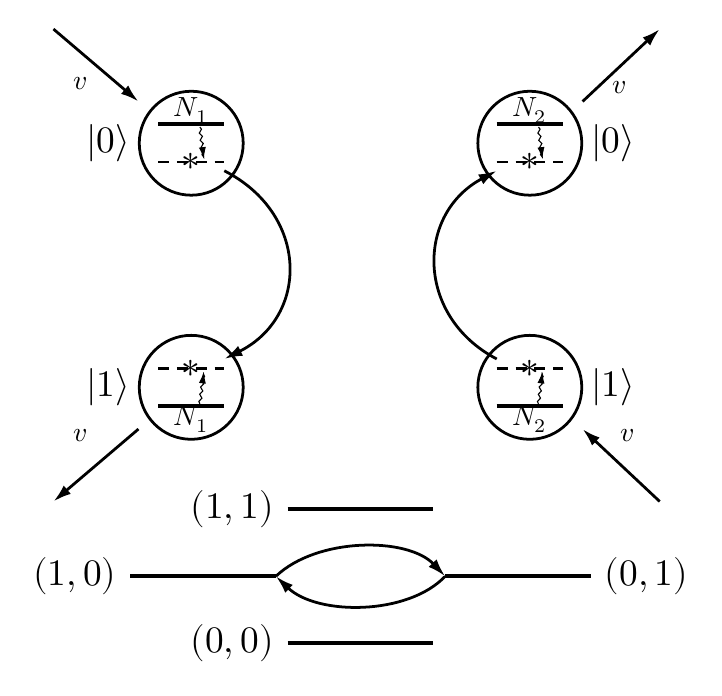
\begin{tikzpicture}[x=1cm,y=1cm]
\coordinate (LT) at (1.60000,5.60000);
\draw[link] (1.60000,5.60000) circle (.66cm);
\draw[lev] (1.18000,5.84000) -- (2.02000,5.84000);
\draw[bare] (1.18000,5.36000) -- (2.02000,5.36000);
\node[small,font=\fontsize{10}{12}\selectfont] at (1.60000,6.01000) {$N_1$};
\node[lab] at (1.60000,5.36000) {$\ast$};
\draw[black,-{Latex[length=1.5mm,width=.9mm]},decorate,decoration={snake,amplitude=.17mm,segment length=.92mm}] (1.71000,5.80500) -- (1.76000,5.40000);
\node[lab,anchor=east] at (0.90000,5.60000) {$|0\rangle$};
\coordinate (LB) at (1.60000,2.50000);
\draw[link] (1.60000,2.50000) circle (.66cm);
\draw[lev] (1.18000,2.26000) -- (2.02000,2.26000);
\draw[bare] (1.18000,2.74000) -- (2.02000,2.74000);
\node[small,font=\fontsize{10}{12}\selectfont] at (1.60000,2.09000) {$N_1$};
\node[lab] at (1.60000,2.74000) {$\ast$};
\draw[black,-{Latex[length=1.5mm,width=.9mm]},decorate,decoration={snake,amplitude=.17mm,segment length=.92mm}] (1.71000,2.29000) -- (1.76000,2.70000);
\node[lab,anchor=east] at (0.90000,2.50000) {$|1\rangle$};
\coordinate (RT) at (5.90000,5.60000);
\draw[link] (5.90000,5.60000) circle (.66cm);
\draw[lev] (5.48000,5.84000) -- (6.32000,5.84000);
\draw[bare] (5.48000,5.36000) -- (6.32000,5.36000);
\node[small,font=\fontsize{10}{12}\selectfont] at (5.90000,6.01000) {$N_2$};
\node[lab] at (5.90000,5.36000) {$\ast$};
\draw[black,-{Latex[length=1.5mm,width=.9mm]},decorate,decoration={snake,amplitude=.17mm,segment length=.92mm}] (6.01000,5.80500) -- (6.06000,5.40000);
\node[lab,anchor=west] at (6.60000,5.60000) {$|0\rangle$};
\coordinate (RB) at (5.90000,2.50000);
\draw[link] (5.90000,2.50000) circle (.66cm);
\draw[lev] (5.48000,2.26000) -- (6.32000,2.26000);
\draw[bare] (5.48000,2.74000) -- (6.32000,2.74000);
\node[small,font=\fontsize{10}{12}\selectfont] at (5.90000,2.09000) {$N_2$};
\node[lab] at (5.90000,2.74000) {$\ast$};
\draw[black,-{Latex[length=1.5mm,width=.9mm]},decorate,decoration={snake,amplitude=.17mm,segment length=.92mm}] (6.01000,2.29000) -- (6.06000,2.70000);
\node[lab,anchor=west] at (6.60000,2.50000) {$|1\rangle$};
\draw[ray] (2.02000,5.25000) .. controls (3.10000,4.70000) and (3.10000,3.40000) .. (2.02000,2.86000);
\draw[ray] (5.48000,2.86000) .. controls (4.45000,3.40000) and (4.45000,4.70000) .. (5.48000,5.25000);
\draw[ray] (-0.15000,7.05000) -- (0.93000,6.13000);
\draw[ray] (0.93000,1.97000) -- (-0.15000,1.05000);
\draw[ray] (7.55000,1.05000) -- (6.57000,1.97000);
\draw[ray] (6.57000,6.13000) -- (7.55000,7.05000);
\node[small,font=\fontsize{10}{12}\selectfont] at (0.20000,6.32000) {$v_{\mathrm{отн}}$};
\node[small,font=\fontsize{10}{12}\selectfont] at (0.20000,1.85000) {$v_{\mathrm{отн}}$};
\node[small,font=\fontsize{10}{12}\selectfont] at (7.15000,1.85000) {$v_{\mathrm{отн}}$};
\node[small,font=\fontsize{10}{12}\selectfont] at (7.05000,6.27000) {$v_{\mathrm{отн}}$};
\coordinate (C11) at (3.75000,0.95000);
\coordinate (C11L) at (2.82500,0.95000);
\coordinate (C11R) at (4.67500,0.95000);
\draw[lev] (C11L) -- (C11R);
\node[lab,anchor=east] at (2.72500,0.95000) {$(1,1)$};
\coordinate (C00) at (3.75000,-0.75000);
\coordinate (C00L) at (2.82500,-0.75000);
\coordinate (C00R) at (4.67500,-0.75000);
\draw[lev] (C00L) -- (C00R);
\node[lab,anchor=east] at (2.72500,-0.75000) {$(0,0)$};
\coordinate (C10) at (1.75000,0.10000);
\coordinate (C10L) at (0.82500,0.10000);
\coordinate (C10R) at (2.67500,0.10000);
\draw[lev] (C10L) -- (C10R);
\node[lab,anchor=east] at (0.72500,0.10000) {$(1,0)$};
\coordinate (C01) at (5.75000,0.10000);
\coordinate (C01L) at (4.82500,0.10000);
\coordinate (C01R) at (6.67500,0.10000);
\draw[lev] (C01L) -- (C01R);
\node[lab,anchor=west] at (6.77500,0.10000) {$(0,1)$};
\draw[ray] (C10R) .. controls (3.20000,0.60000) and (4.35000,0.60000) .. (C01L);
\draw[ray] (C01L) .. controls (4.35000,-0.40000) and (3.20000,-0.40000) .. (C10R);\end{tikzpicture}

\end{document}
